\section{Planiranje}

\textbf{plan} zaporedje akcij, ki pripelje od zacetnega do koncnega stanja

\subsection{STRIPS}
Agentu opisemo svet in postavimo fizikalne omejitve.\\
Ne zagotovalja optimalne resitve, obravnavamo le en cilj naenkrat (ko ga dosezemo, se lahko ostali izgubijo) = Sussmanova anomalija\\
\green{Akcija} move(X, From, To)
\begin{itemize}[noitemsep,topsep=0pt,leftmargin=*]
    \item \blue{pogoj}: con=[clr(X), on(X,F), clr(T)] $\rightarrow$ pogoji za izvajanje akcije,
    \item \blue{poz. ucinki}: adds=[on(X, T), clr(F)] $\rightarrow$ nova stanja,
    \item \blue{neg. ucinki}: dels=[on(X, F), clr(T)] $\rightarrow$ izbrisana stanja,
    \item \blue{omejitve}: constr=[F $\neq$ T, X$\neq$ F, X$\neq$ T, block(X)] $\rightarrow$ omejitve akcij (fizikalne omejitve),
\end{itemize}
\cyan{Algoritem}:
\begin{enumerate}[noitemsep,topsep=0pt,leftmargin=*]
    \item Izberi se neresen cilj iz mnozice CILJEV
    \item Izberi akcijo, ki izbrani cilj doda v stanje
    \item Omogoci izbrano akcijo (izpolni pogoje)
    \item Izvedi akcijo (ki izopolni najvec pogojev)
    \item Ce obstajajo nereseni cilji $\Rightarrow$ 1.
\end{enumerate}
\magenta{Primer dfs, zlaganje kock}

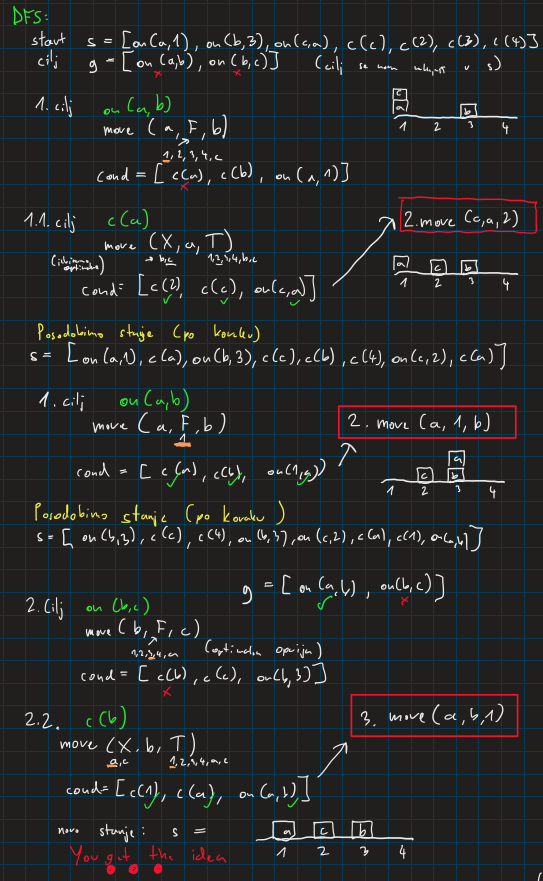
\includegraphics[trim={0cm 0cm 0cm 0cm},clip,width=6.5cm]{strips.png}



\subsection{PLANIRANJE Z REGRESIRANJEM CILJEV}
Resitev za sussmanovo anomalijo

\subsection{RAZPOREJANJE OPRAVIL}

